%\documentclass[handout]{beamer}
\documentclass[compress]{beamer}

%\documentclass{beamer}
\usepackage[T1]{fontenc}
\usepackage{pifont}
\usepackage{threeparttable}
\usepackage{subcaption}
\usepackage{tikz-qtree}
\usepackage{listings}
\usepackage[american]{babel}
\usepackage{csquotes}
\usepackage[style=apa, backend=biber]{biblatex}
\usepackage{tikz}
\usepackage{multicol}
\usepackage{booktabs}
\usepackage{graphicx}
\usepackage{neuralnetwork}
\usepackage{hyperref}

\usepackage{minted}
\definecolor{listingbg}{rgb}{0.87,0.93,1}
\setminted[python]{
breaklines,
linenos,
fontsize=\scriptsize,
frame=single,
xleftmargin=0pt}

\hypersetup{
    pdfborder={0 0 0},
    colorlinks=true,
}
\usetheme[block=fill,subsectionpage=progressbar,sectionpage=progressbar]{metropolis} 

\definecolor{Purple}{HTML}{911146}
\definecolor{Orange}{HTML}{CF4A30}

\setbeamercolor{alerted text}{fg=Orange}
\setbeamercolor{frametitle}{bg=Purple}

\setbeamercovered{still covered={\opaqueness<1->{5}},again covered={\opaqueness<1->{100}}}

\lstset{
    basicstyle=\scriptsize\ttfamily,
    columns=flexible,
    breaklines=true,
    numbers=left,
    %stepsize=1,
    numberstyle=\tiny,
    backgroundcolor=\color[rgb]{0.85,0.90,1}
}

\lstnewenvironment{lstlistingoutput}{\lstset{
        basicstyle=\footnotesize\ttfamily,
        columns=flexible,
        breaklines=true,
        numbers=left,
        %stepsize=1,
        numberstyle=\tiny,
        backgroundcolor=\color[rgb]{.7,.7,.7}}}{}


\lstnewenvironment{lstlistingoutputtiny}{\lstset{
        basicstyle=\tiny\ttfamily,
        columns=flexible,
        breaklines=true,
        numbers=left,
        %stepsize=1,
        numberstyle=\tiny,
        backgroundcolor=\color[rgb]{.7,.7,.7}}}{}

\renewcommand*{\bibfont}{\tiny}

\makeatletter
\setbeamertemplate{headline}{%
    \begin{beamercolorbox}[colsep=1.5pt]{upper separation line head}
    \end{beamercolorbox}
    \begin{beamercolorbox}{section in head/foot}
        \vskip2pt\insertnavigation{\paperwidth}\vskip2pt
    \end{beamercolorbox}%
    \begin{beamercolorbox}[colsep=1.5pt]{lower separation line head}
    \end{beamercolorbox}
}
\makeatother

\newcommand{\question}[1]{
    \begin{frame}[plain]
        \begin{columns}
            \column{.4\textwidth}
            \makebox[\columnwidth]{
                
\includegraphics[width=\columnwidth,height=\paperheight,keepaspectratio]{../pictures/mannetje.png}}
            \column{.6\textwidth}
            \large
            \textcolor{orange}{\textbf{\emph{#1}}}
        \end{columns}
    \end{frame}}

\newcommand{\instruction}[1]{\emph{\textcolor{gray}{[#1]}}}

\addbibresource{../resources/literature.bib}
\graphicspath{{../resources/pictures/}}

\title[Computational Communication Science 2]{\textbf{Computational Communication Science 2} \\Week 3 - Lecture\\ »Bottom up approaches to text analysis«}
\author[Anne Kroon]{Anne Kroon \\ ~ \\ \footnotesize{ a.c.kroon@uva.nl, @annekroon} \\}
\date{April 17, 2023}
\institute[Digital Society Minor, University of Amsterdam]{Digital Society Minor, University of Amsterdam}

\begin{document}
	
	\begin{frame}{}
		\titlepage
	\end{frame}
	
	\begin{frame}{Today}
		\begin{tiny}
		\tableofcontents
		\end{tiny}
	\end{frame}

\input{../modules/vectorizers_main}



\section{Cosine Similarity}

\begin{frame}{Cosine Similarity}
	\begin{block}{Cosine Similarity}
		\begin{itemize}[<+>]
			\item A measure that helps you determine how similar two documents are, irrespective of their size
		\end{itemize}
	
		\begin{exampleblock}{Applications in Communication Science}
		\begin{itemize}[<+>]
			\item For example, to map \emph{linguistic alignment} of romantic couples over time \textcite{Brinberg2021} 
			\item Or, in the political domain, agenda overlap between public opinion and political speech \textcite{Hager2020}
		\end{itemize}
	\end{exampleblock}
	\end{block}
\end{frame}

\begin{frame}{Cosine Similarity} 
$$
\text { similarity }=\cos (\theta)=\frac{\mathbf{A} \cdot \mathbf{B}}{\|\mathbf{A}\|\|\mathbf{B}\|}=\frac{\sum_{i=1}^{n} A_{i} B_{i}}{\sqrt{\sum_{i=1}^{n} A_{i}^{2}} \sqrt{\sum_{i=1}^{n} B_{i}^{2}}}
$$

\pause

\begin{itemize}[<+>]
\item It measures the cosine of the angle between two vectors projected in a multi-dimensional space.
\item 0 means orthogonal vectors (90 degrees); very dissimal
\item 1 means vectors are the same (0 degrees); similar
\end{itemize}
\end{frame}


\begin{frame}{Cosine Similarity}
	\makebox[\columnwidth]{
		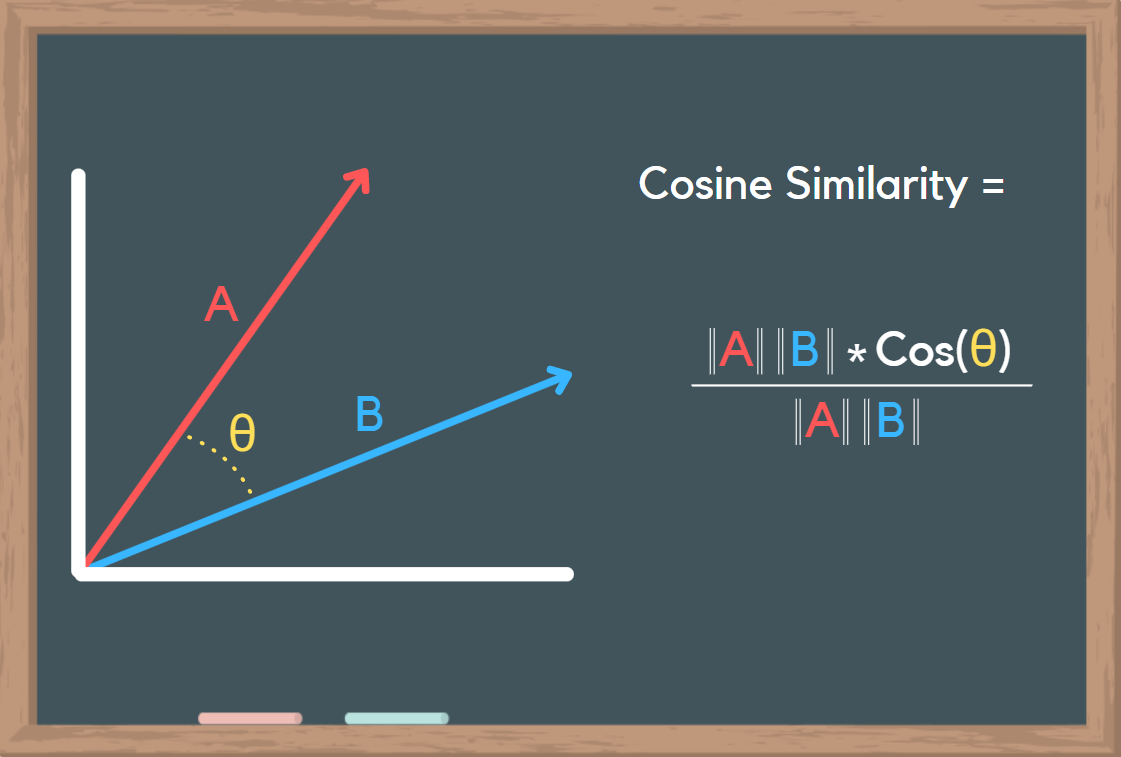
\includegraphics[width=\columnwidth,height=\paperheight,keepaspectratio]{cosine_angle.png}}
	\\
\footnote{https://towardsdatascience.com/what-is-cosine-similarity-how-to-compare-text-and-images-in-python-d2bb6e411ef0}
\end{frame}



% recommender systems are everywhere around us.
\begin{frame}{how can we calculate this in python?}
Let's review a practical application \footnote{https://github.com/uva-cw-ccs2/2223s2/blob/master/week03/exercises/OPTIONAL_overtime_similarity.ipynb}.
\end{frame}


\begin{frame}[fragile, plain]
	\begin{minted}[%
		breaklines,
		linenos,
		fontsize=\scriptsize,
		frame=single,
		xleftmargin=0pt,]
		{python}
from sklearn.feature_extraction.text import CountVectorizer, TfidfVectorizer
import pandas as pd

doc1 = "When I eat breakfast, I usually drink some tea".lower()
doc2 = "I like my tea with my breakfast".lower()
doc3 = "She likes cereal and coffee".lower()

vec = CountVectorizer(stop_words='english')
count_matrix = vec.fit_transform([doc1, doc2, doc3])

print(pd.DataFrame(count_matrix.A, columns=vec.get_feature_names()).to_string())
\end{minted}

\pause
%\begin{lstlistingoutput}
\begin{minted}[fontsize=\scriptsize]{python}
     breakfast  cereal  coffee  drink  eat  like  likes  tea  usually
0          1       0       0      1    1     0      0    1        1
1          1       0       0      0    0     1      0    1        0
2          0       1       1      0    0     0      1    0        0
\end{minted}
%\end{lstlistingoutput}s
\end{frame}

\begin{frame}[fragile]{Implementation in Python}
	\begin{minted}[%
		breaklines,
		linenos,
		fontsize=\scriptsize,
		frame=single,
		xleftmargin=0pt,]
		{python}
doc1_vector = pd.DataFrame(count_matrix.A, columns=vec.get_feature_names()).T[0].to_list()
doc2_vector = pd.DataFrame(count_matrix.A, columns=vec.get_feature_names()).T[1].to_list()

print(f"The vector belonging to doc1: {doc1_vector}")
print(f"The vector belonging to doc2: {doc2_vector}")
	\end{minted}
	
	\pause
	%\begin{lstlistingoutput}
	\begin{minted}{python}
The vector belonging to doc1: [1, 0, 0, 1, 1, 0, 0, 1, 1]
The vector belonging to doc2: [1, 0, 0, 0, 0, 1, 0, 1, 0]
	\end{minted}
	%\end{lstlistingoutput}s
\end{frame}


\begin{frame}[fragile]{Implementation in Python}
Now, lets populate the formula.
1.Execute the part of the formula in the numerator. Specifically, take the dot product of the vectors:
$$
\sum_{i=1}^{n} A_{i} B_{i}
$$

\begin{minted}[fontsize=\scriptsize]{python}
doc1: [1, 0, 0, 1, 1, 0, 0, 1, 1]
doc2: [1, 0, 0, 0, 0, 1, 0, 1, 0]
\end{minted}
%\end{lstlistingoutput}s
$$
dot\_product = (1\cdot1) + (0\cdot0) + (0\cdot0) + (1\cdot0) + (1\cdot0) + (0\cdot0) + (1\cdot1) +(1\cdot0)
$$
\pause
Or, using Python: 
	\begin{minted}[%
		breaklines,
		linenos,
		fontsize=\scriptsize,
		frame=single,
		xleftmargin=0pt,]
		{python}
dot_product = sum([num1 * num2 for num1, num2 in zip(doc1_vector, doc2_vector)])
print(dot_product)
	\end{minted}
\pause
	%\begin{lstlistingoutput}
	\begin{minted}{python}
2
	\end{minted}
	%\end{lstlistingoutput}s
\end{frame}



\begin{frame}[fragile]{Implementation in Python}
    2.Execute the part of the formula in the denumerator. Take the cross product of the two vectors.

$$
\sqrt{\sum_{i=1}^{n} A_{i}^{2}} \sqrt{\sum_{i=1}^{n} B_{i}^{2}}
$$
\footnotesize{Calculate this by hand:
$$
doc1_ = \sqrt{1^2 + 0^2 + 0^2 + 1^2 + 1^2 + 0^2+ 1^2 + 1^2}
$$
$$
doc1_ = \sqrt{1^2 + 0^2 + 0^2 + 0^2 + 1^2 + 0^2+ 1^2 + 0^2}
$$
}
\pause
Implementation in Python:
	\begin{minted}[%
		breaklines,
		linenos,
		fontsize=\scriptsize,
		frame=single,
		xleftmargin=0pt,]
		{python}
import math
doc1_ = math.sqrt(sum( [i**2 for i in doc1_vector]) )
doc2_ = math.sqrt(sum( [i**2 for i in doc2_vector]) )

doc1_ * doc2_
\end{minted}
	\pause
%\begin{lstlistingoutput}
\begin{minted}{python}
3.872983346207417
\end{minted}
%\end{lstlistingoutput}s
\end{frame}


\begin{frame}[fragile]{Implementation in Python}
	3.Finally:

\begin{minted}[%
	breaklines,
	linenos,
	fontsize=\scriptsize,
	frame=single,
	xleftmargin=0pt,]
	{python}
cos_sim = dot_product / (doc1_ * doc2_)
print(cos_sim)
\end{minted}

\pause

\begin{minted}[fontsize=\scriptsize]{python}
0.5163977794943222
\end{minted}
\end{frame}

\begin{frame}[fragile]{Implementation in Python}

We can, however, do this much faster using sklearn's \texttt{cosine\_similarity}.
	
\begin{minted}[%
	breaklines,
	linenos,
	fontsize=\scriptsize,
	frame=single,
	xleftmargin=0pt,]
	{python}
from sklearn.metrics.pairwise import cosine_similarity
cosine_similarity([doc1_vector, doc2_vector])
\end{minted}
	
	\pause
	
\begin{minted}[fontsize=\scriptsize]{python}
array([[1.        , 0.51639778],
[0.51639778, 1.        ]])
	\end{minted}
\end{frame}

\begin{frame}{How to use this in practice}
	\begin{block}{What can you do with this?}
		\begin{itemize}[<+>]
			\item This is especially powerful if you want to compare different news articles, movies, song texts, etc.
			\item For example, which movies are most similair in terms of genre composition?
			\end{itemize}
	\end{block}
\end{frame}

\begin{frame}
	\makebox[\linewidth]{
		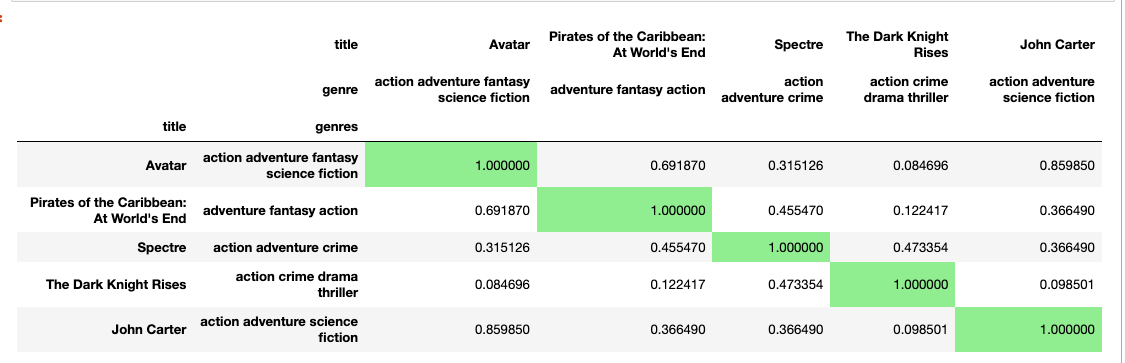
\includegraphics[width=\columnwidth,height=\paperheight,keepaspectratio]{cosine_sim.png}}
Indentify movies that are similar in terms of genre  \footnote{https://www.learndatasci.com/glossary/cosine-similarity/}
\end{frame}

\begin{frame}{Considering Cosine Similarity}
	\begin{block}{Things to consider}
		\begin{itemize}
		\item <1-> What type of overlap are you interested in?
		\item <2->What is the meaning of n-grams, stems,  stopwords when considering your RQ? How you should preproces, depends on your RQ and aim. 
		\item <3-> Computationally cheap and fast; works well in e.g., recommender systems (week 4!)
		\end{itemize}
	\end{block}
\begin{alertblock}{Drawbacks}
	\begin{itemize}
	\item <4-> An \emph{exact} match in terms of words is needed. Is that realistic?	
	\end{itemize}
\end{alertblock}
\end{frame}

\begin{frame}[fragile]{Implementation in Python}
	\begin{minted}[%
		breaklines,
		linenos,
		fontsize=\scriptsize,
		frame=single,
		xleftmargin=0pt,]
		{python}
doc1 = "When I eat breakfast, I usually drink some tea".lower()
doc2 = "I like my tea with my breakfast".lower()
doc3 = "She likes cereal and coffee".lower()
	\end{minted}
	What do you expect here? Should there be some level of overlap?
\end{frame}


\begin{frame}[fragile]{Implementation in Python}
\begin{minted}[%
	breaklines,
	linenos,
	fontsize=\scriptsize,
	frame=single,
	xleftmargin=0pt,]
	{python}
doc1 = "When I eat breakfast, I usually drink some tea".lower()
doc2 = "I like my tea with my breakfast".lower()
doc3 = "She likes cereal and coffee".lower()
\end{minted}
	
\begin{minted}[%
	breaklines,
	linenos,
	fontsize=\scriptsize,
	frame=single,
	xleftmargin=0pt,]
	{python}
print(cosine_similarity([doc1_vector, doc2_vector, doc3_vector]))
\end{minted}
	\pause
\begin{minted}[fontsize=\scriptsize]{python}
[[1.         0.51639778 0.        ]
[0.51639778 1.         0.        ]
[0.         0.         1.        ]]
\end{minted}
	\pause
Zero overlap between doc3 and the other documents. Is that correct?
\end{frame}


\section{Soft cosine similarity}

\begin{frame}{Soft cosine similarity}
	\huge{...enter soft cosine similarty} \textcite{Sidorov2014}\\
	\pause
	\footnotesize{``Soft Cosine Measure (SCM) is a method that allows us to assess the similarity between two documents in a meaningful way, even when they have no words in common. It uses a measure of similarity between words, which can be derived using [word2vec] vector embeddings of words.''}
	\footnote{\url{https://radimrehurek.com/gensim//auto_examples/tutorials/run_scm.html}}
\end{frame}

\begin{frame}{Soft Cosine Measure (SCM)}
	\begin{block}{SCM}
		\begin{itemize}
			\item <1-> Even if two sentences do not share the same words, we can calculate similarity by modelling \emph{synonym}
			\item <2->For example, the words `play' and `game' are different but related \textcite{Sidorov2014} \footnote{\url{http://www.scielo.org.mx/pdf/cys/v18n3/v18n3a7.pdf}}
			\item<3->How can we capture `semantic' meaning?
		\end{itemize}
	\end{block}
	\begin{exampleblock}{How?}
		\begin{itemize}
			\item <4-> Convert words to \emph{word vectors} and then compute similarities  \footnote{\url{https://www.machinelearningplus.com/nlp/cosine-similarity/}}
		\end{itemize}
	\end{exampleblock}
\end{frame}


\begin{frame}
	\makebox[\linewidth]{
		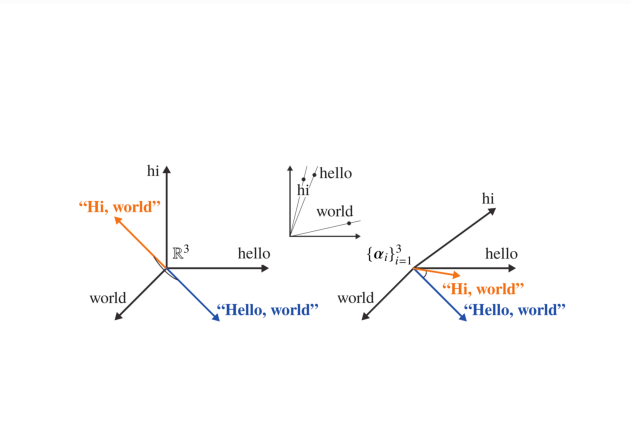
\includegraphics[width=\columnwidth,height=\paperheight,keepaspectratio]{soft-cosine}}
	Soft cosine similarity \footnote{\url{https://radimrehurek.com/gensim//auto_examples/tutorials/run_scm.html}}
\end{frame}

\begin{frame}{Word embeddings}
	\begin{block}{Word embeddings}
		\begin{itemize}
			\item <1->To use the SCM, you need word embeddings. 
		\end{itemize}
	\end{block}
\end{frame}

\subsection{Word embeddings}

\begin{frame}{Understanding SCM}
SCM estimates extracts similarity from \alert{word embeddings}. 
	\begin{block}{What are word embeddings?}
		\begin{itemize}[<+>]
			\item No technical details here, just the general idea
			\item Word embeddings help capturing the meaning of text
			\item Word embeddings are low-dimensional vector representations that capture semantic meaning
			\item State-of-the-art in NLP...
			\item \emph{``...a word is characterized by the company it keeps...''} (Firth, 1957)
		\end{itemize}
	\end{block}
\end{frame}

\iffalse
\begin{frame}{}
	\makebox[\linewidth]{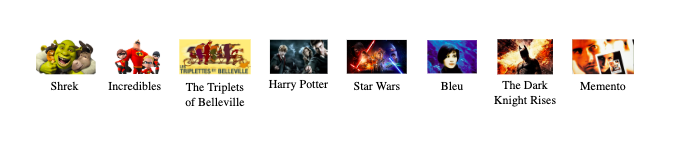
\includegraphics[width=\linewidth,height=\textheight, keepaspectratio]{google1.png}}
\end{frame}

\begin{frame}{}
	\makebox[\linewidth]{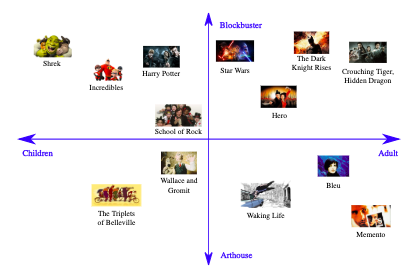
\includegraphics[width=\linewidth,height=\textheight, keepaspectratio]{google2.png}}
\end{frame}


\begin{frame}{}
	\makebox[\linewidth]{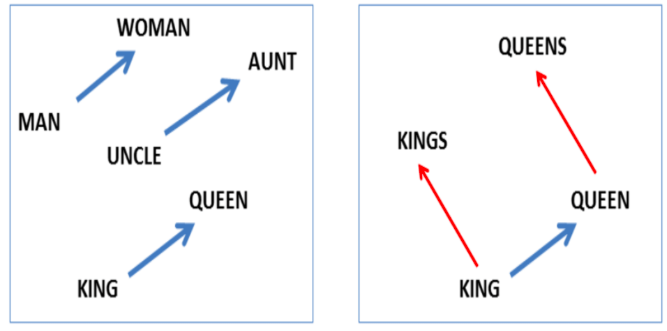
\includegraphics[width=\linewidth,height=\textheight, keepaspectratio]{embeddings.png}}
	
	$king-man+woman = ?$ 
\end{frame}


\begin{frame}{}
	\makebox[\linewidth]{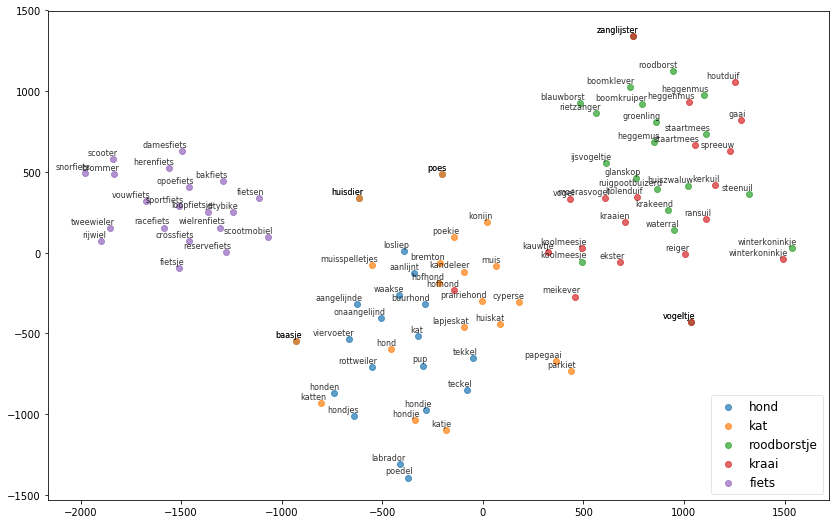
\includegraphics[width=\linewidth,height=\textheight, keepaspectratio]{w2v_300_illustration.png}}
\end{frame}


\begin{frame}{}
	\makebox[\linewidth]{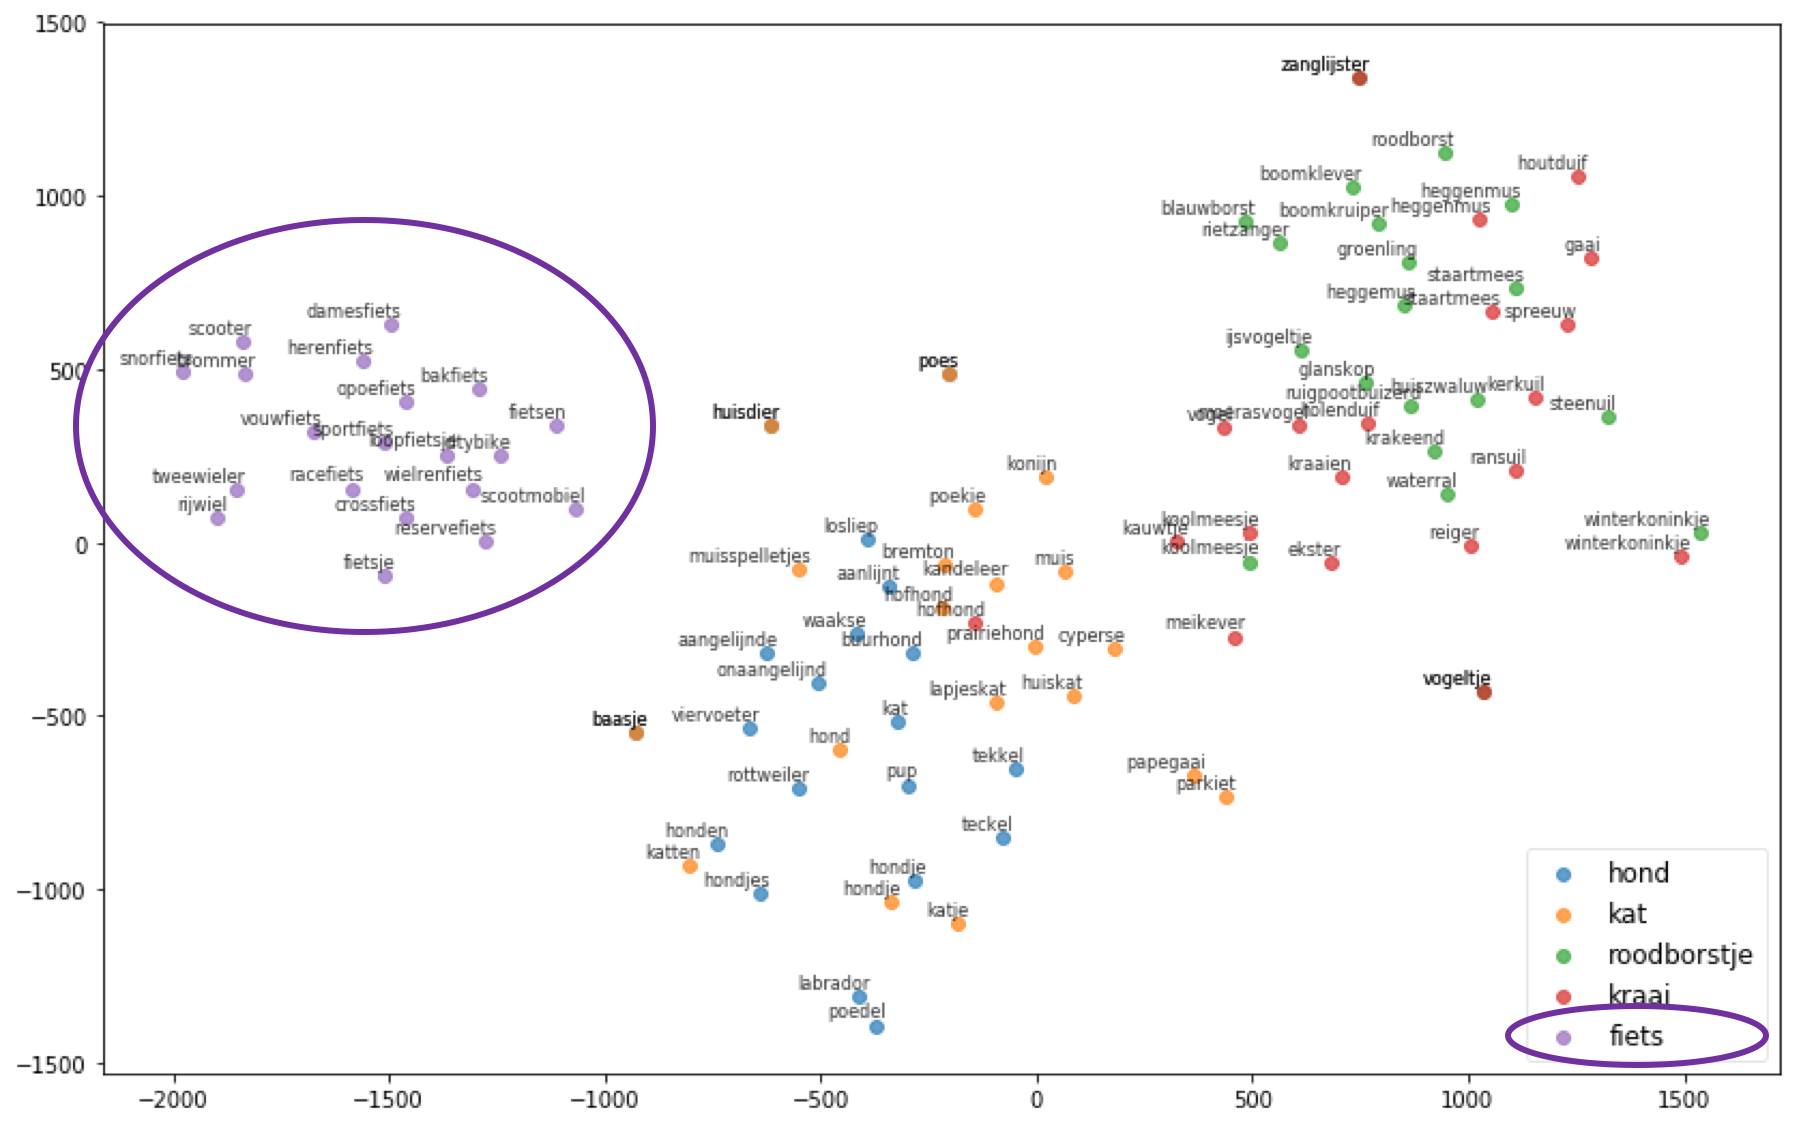
\includegraphics[width=\linewidth,height=\textheight, keepaspectratio]{visual2.png}}
\end{frame}

%as can be seen, words most similar to fiets are on the left. 

\begin{frame}{}
	\makebox[\linewidth]{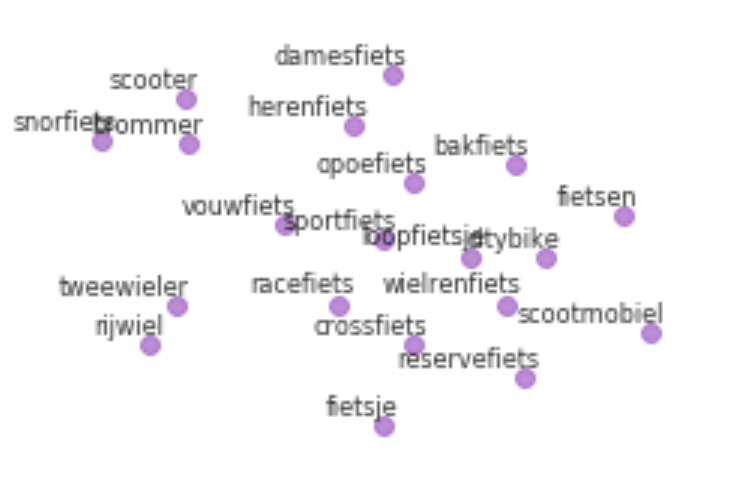
\includegraphics[width=\linewidth,height=\textheight, keepaspectratio]{fiets}}
\end{frame}

%the model has learned that fiets is similar to racefiets, wielrenfiets, rijwiel - and different from the animal department: it doesnt overlap with our kats/ dogs and birds clusters

\begin{frame}{}
	\makebox[\linewidth]{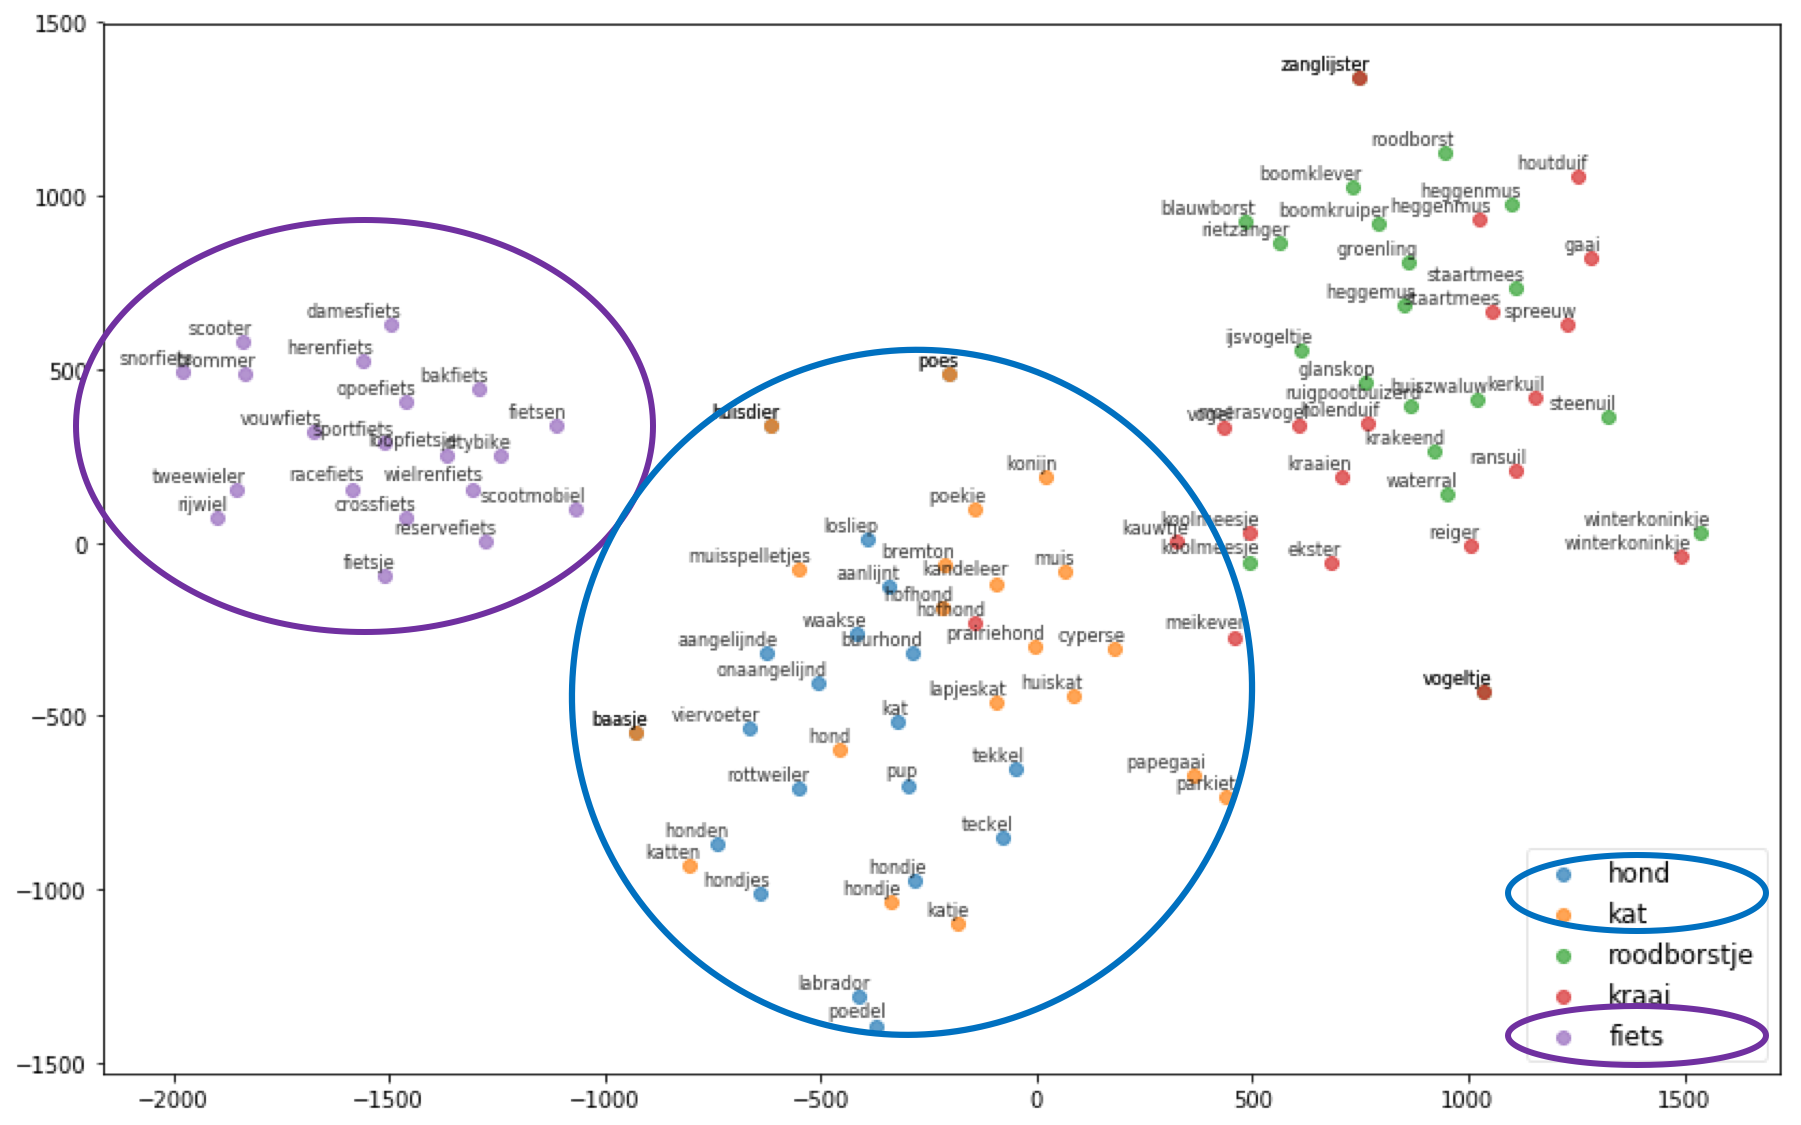
\includegraphics[width=\linewidth,height=\textheight, keepaspectratio]{visual1.png}}
\end{frame}

%the model recognizes that fiets is something else from honden and katten. Both mammals and pets, dogs and cats are quite similar and appear in the same cluster.  

\begin{frame}{}
	\makebox[\linewidth]{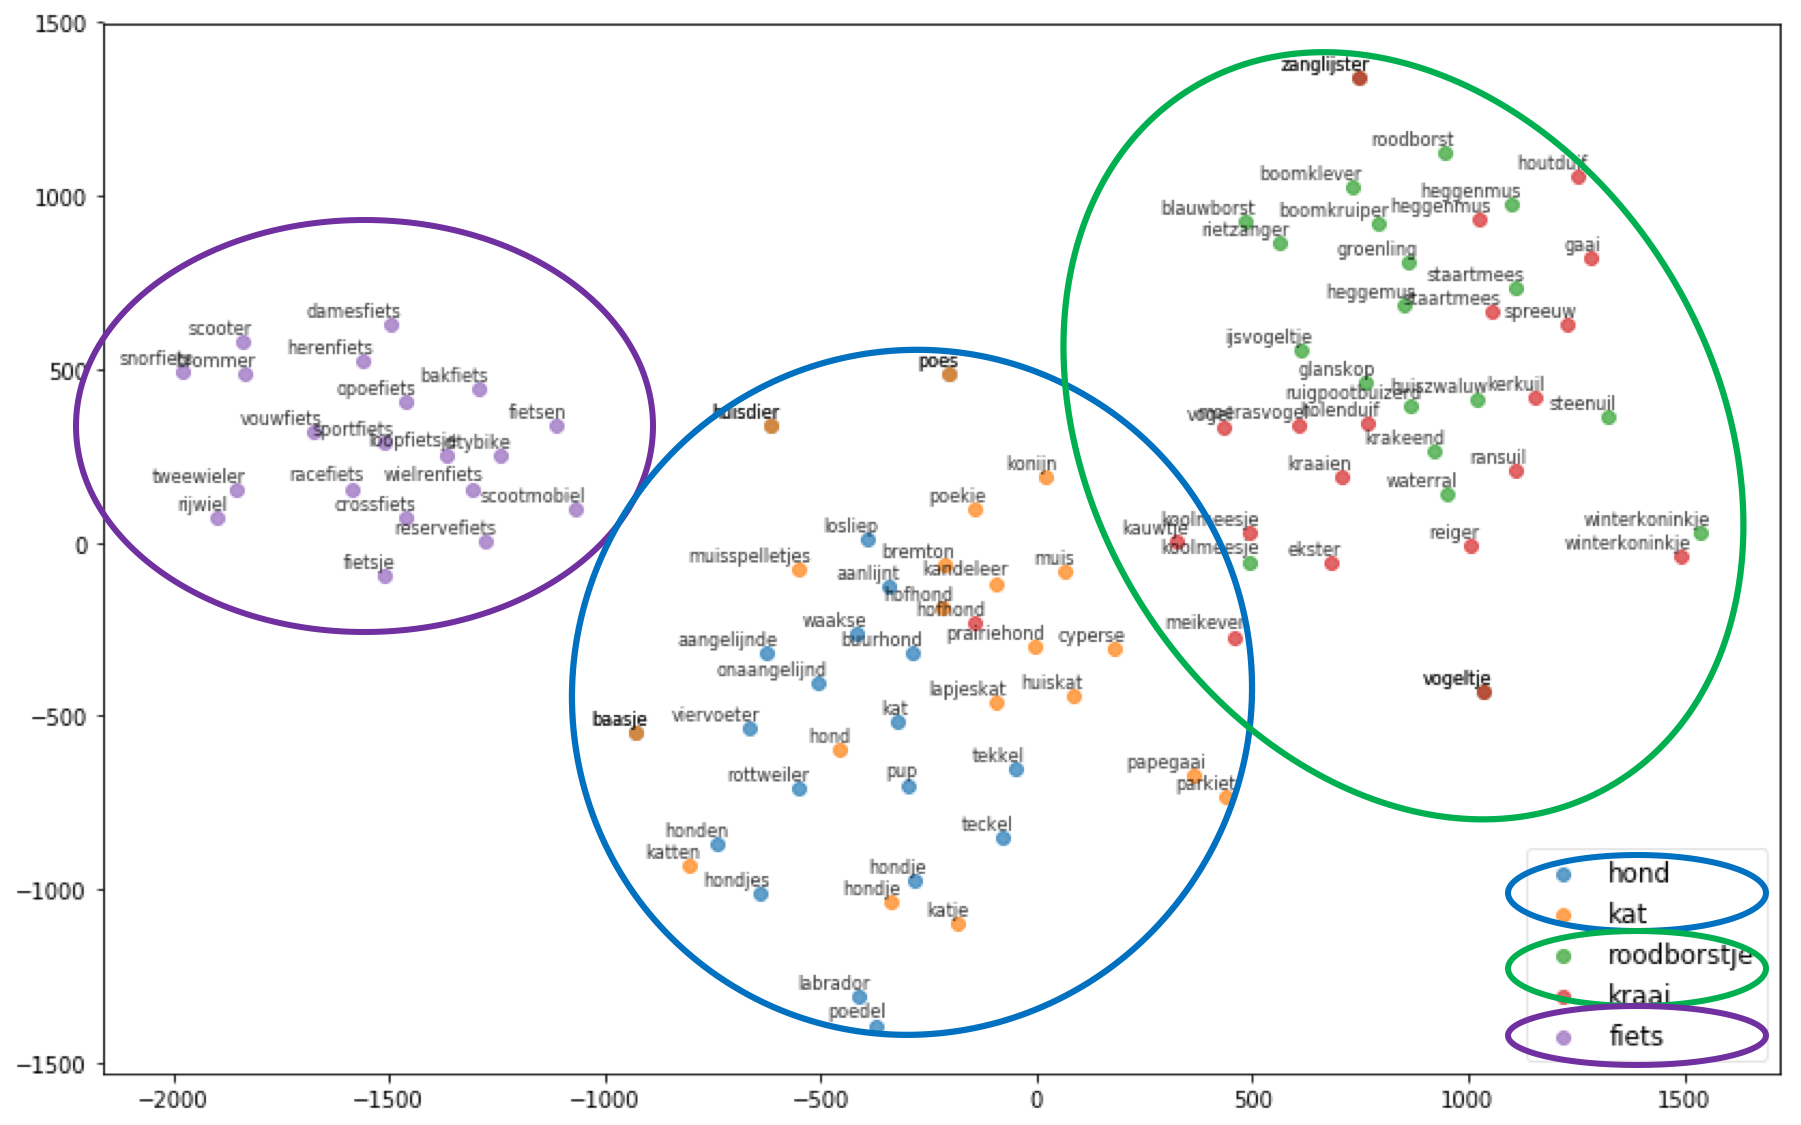
\includegraphics[width=\linewidth,height=\textheight, keepaspectratio]{visual.png}}
\end{frame}
\fi



\subsection{Implemention in Python}
\begin{frame}[fragile]{SCM in Python}
	\begin{block}{Calculating Soft Cosine Measure}
		\begin{itemize}
			\item<1->To use the SCM, you need embeddings. 
			\item<2-> We \emph{can} train embeddings on our own corpus (if we had a lot of data) \dots
			\item<3-> But for now we will use pre-trained models \footnote{\url{https://github.com/uva-cw-ccs2/2223s2/blob/master/week03/exercises/cosine-similarity-basics.ipynb}}. \dots
		\end{itemize}
	\end{block}
\pause
\pause
\pause
\begin{minted}[%
	breaklines,
	fontsize=\scriptsize,
	frame=single,
	xleftmargin=0pt,]
	{python}
import gensim.downloader as api
	
fasttext_model300 = api.load('fasttext-wiki-news-subwords-300')
\end{minted}
\end{frame}

\begin{frame}[fragile]{Create a dictionary}	
\footnotesize{Let's review our 3 documents:}
\begin{minted}[%
breaklines,
linenos,
fontsize=\tiny,
frame=single,
xleftmargin=0pt,]
	{python}
doc1 = "When I eat breakfast, I usually drink some tea".lower()
doc2 = "I like my tea with my breakfast".lower()
doc3 = "She likes cereal and coffee".lower()	
\end{minted}
\pause
\footnotesize{Initialize a Dictionary. This step assigns a \texttt{token\_id} to each word:}
\begin{minted}[%
breaklines,
linenos,
fontsize=\tiny,
frame=single,
xleftmargin=0pt,]
{python}
from gensim.utils import simple_preprocess
from gensim.corpora import Dictionary
dictionary = corpora.Dictionary([simple_preprocess(doc) for doc in [doc1, doc2, doc3]]) 
\end{minted}
\pause
\footnotesize{Now, let's check whether a specific word--for example \texttt{coffee}--is in our \texttt{dictionary:}}
\begin{minted}[%
breaklines,
linenos,
fontsize=\tiny,
frame=single,
xleftmargin=0pt,]
	{python}
'coffee' in dictionary.token2id
\end{minted}
	\pause
	%\begin{lstlistingoutput}
	\begin{minted}{python}
True
	\end{minted}
\end{frame}


\begin{frame}[fragile]{Create a bag-of-words representation}	
\footnotesize{Next, let's represent each document by \texttt{(token\_id, token\_count)} tuples}:
\begin{minted}[%
breaklines,
linenos,
fontsize=\scriptsize,
frame=single,
xleftmargin=0pt,]
{python}
bag_of_words_vectors = [ dictionary.doc2bow(simple_preprocess(doc)) for doc in [doc1, doc2, doc3]] 
\end{minted}
\pause
\footnotesize{Build a term similarity matrix and compute a sparse term similarity matrix}:
\begin{minted}[%
	breaklines,
	linenos,
	fontsize=\scriptsize,
	frame=single,
	xleftmargin=0pt,]
	{python}
from gensim.similarities import SparseTermSimilarityMatrix
from gensim.similarities import WordEmbeddingSimilarityIndex

similarity_index = WordEmbeddingSimilarityIndex(fasttext_model300)
similarity_matrix = SparseTermSimilarityMatrix(similarity_index, dictionary)
\end{minted}
\end{frame}

\begin{frame}[fragile]{Inspect results}	
	\footnotesize{Get SCM using \texttt{.inner\_product()}: }:
	\begin{minted}[%
		breaklines,
		linenos,
		fontsize=\tiny,
		frame=single,
		xleftmargin=0pt,]
		{python}
#between doc1 and doc2:
scm_doc1_doc2 = similarity_matrix.inner_product(bag_of_words_vectors[0], bag_of_words_vectors[1], normalized=(True, True))

#between doc1 and doc3:
scm_doc1_doc3 = similarity_matrix.inner_product(bag_of_words_vectors[0], bag_of_words_vectors[2], normalized=(True, True))

#between doc2 and doc3;
scm_doc2_doc3 = similarity_matrix.inner_product(bag_of_words_vectors[1], bag_of_words_vectors[2], normalized=(True, True))

print(f"SCM between:\ndoc1 <-> doc2: {scm_doc1_doc2:.2f}\ndoc1 <-> doc3: {scm_doc1_doc3:.2f}\ndoc2 <-> doc3: {scm_doc2_doc3:.2f}")
	\end{minted}
	\pause
	\footnotesize{Do the results make more sense?}:
	\begin{minted}[%
		fontsize=\tiny,]
		{python}
SCM between:
doc1 <-> doc2: 0.29
doc1 <-> doc3: 0.15
doc2 <-> doc3: 0.28
\end{minted}
\end{frame}
	
\begin{frame}{Applications of cosine and soft cosine similarity}
	Applications of \emph{cosine} and \emph{soft cosine} in the field of Communication Science generally involve some overtime dynamics. 
	\begin{exampleblock}{Trace convergence or agenda setting dynamics over time}
		\begin{itemize}
			\item Beyond the scope this course to discuss it here, but if you are interested in how you can apply cosine and soft cosine in an overtime analysis, we have prepared a notebook that will help you do just that. 
			\item \url{https://github.com/uva-cw-ccs2/2223s2/main/week03/exercises/OPTIONAL_overtime_similarity.ipynb}
		\end{itemize}
	\end{exampleblock}

\end{frame}

\section{From test to large-scale}

\begin{frame}[fragile]{General approach}
1. Take a single string and test your idea
\begin{minted}[%
	breaklines,
	linenos,
	fontsize=\scriptsize,
	frame=single,
	xleftmargin=0pt,]
	{python}
t = "This is a test test test."
print(t.count("test"))
\end{minted}
2a. You'd assume it to return 3. If so, scale it up:
\pause
\begin{minted}[%
	breaklines,
	linenos,
	fontsize=\scriptsize,
	frame=single,
	xleftmargin=0pt,]
	{python}
results = []
for t in listwithallmytexts:
    r = t.count("test")
    print(f"{t} contains the substring {r} times")
	results.append(r)
\end{minted}

2b. If you \emph{only} need to get the list of results, a list comprehension is more elegant:
\begin{minted}[%
	breaklines,
	linenos,
	fontsize=\scriptsize,
	frame=single,
	xleftmargin=0pt,]
	{python}
results = [t.count("test") for t in listwithallmytexts]
\end{minted}


\end{frame}

\begin{frame}[fragile]{General approach}
\Large

\textcolor{red}{Test on a single string, then make a for loop or list comprehension!}

\pause

\normalsize

\begin{alertblock}{Own functions}
	If it gets more complex, you can write your ow= function and then use it in the list comprehension:
\begin{minted}[%
	breaklines,
	linenos,
	fontsize=\scriptsize,
	frame=single,
	xleftmargin=0pt,]
	{python}
def mycleanup(t):
     # do sth with string t here, create new string t2
     return t2
		
results = [mycleanup(t) for t in allmytexts]
\end{minted}
\end{alertblock}
\end{frame}


\begin{frame}[fragile]{Pandas string methods as alternative}
If you select column with strings from a pandas dataframe, pandas offers a collection of string methods (via \texttt{.str.}) that largely mirror standard Python string methods:

\begin{minted}[%
	breaklines,
	linenos,
	fontsize=\scriptsize,
	frame=single,
	xleftmargin=0pt,]
	{python}
df['newcoloumnwithresults'] = df['columnwithtext'].str.count("bla")
\end{minted}


\pause

\begin{alertblock}{To pandas or not to pandas for text?}
	Partly a matter of taste. 
	
	Not-too-large dataset with a lot of extra columns? Advanced statistical analysis planned? Sounds like pandas.
	
	It's mainly a lot of text? Wanna do some machine learning later on anyway? It's large and (potentially) messy? Doesn't sound like pandas is a good idea.
\end{alertblock}

\end{frame}


\begin{frame}{Thank you!!}
	\begin{block}{Thank you for your attention!}
		\begin{itemize}
			\item Questions? Comments?
		\end{itemize}
	\end{block}
\end{frame}


\begin{frame}
	\frametitle{References}
	\printbibliography
\end{frame}
	

\end{document}